\documentclass[12pt]{ruthesis}
%\documentclass[12pt]{amsart}
\usepackage{amsmath}
\usepackage{amssymb}
\usepackage{latexsym}
\usepackage{epsfig,epsf,rotating}
\usepackage{subfigure}
\usepackage{siunitx}
%\usepackage{pictex}
\usepackage{epsf}
\usepackage{theorem}
\usepackage{graphicx}
\usepackage{hyperref}
\usepackage{typedref}
\usepackage[version=4]{mhchem}
%\usepackage{cite}
\usepackage[numbers, sort&compress]{natbib}

\title{Microwave spectroscopy on two dimensional electron gas}
\ctitle{Microwave spectroscopy on two dimensional electron gas}
\author{Jie Zhang}
\department{Physics and Astronomy}
\school{Rice University}
\degree{Master of Science}

\committee {
		Rui-Rui Du, Chair\\
        Professor of Physics and Astronomy \and
        Junichiro Kono \\
        Professor of Electrical and Computer Engineering and Physics \& Astronomy \and
        Wei Li\\
        Associate Professor of Physics and Astronomy\and
       }

\address{Houston, Texas}
\donemonth{August} \doneyear{2015} \makeindex
\begin{document}

  \begin{frontmatter}
   \pagenumbering{roman}
   %\makecover
   \maketitle

\begin{abstract}

Microwave spectroscopy for detecting various resonance  of electrons is our main focus and we have been using electrical, thermal and absorption method for different purposes.

Electron spin resonance (ESR) and cyclotron resonance (CR) are two of the most significant feature of electrons under magnetic field where electrical detection requires contacts on the sample which usually causes damages.
In order to detect the ESR of a single nano-object, high sensitive tool is required.
So far, the best commercial ESR detector can detect around 1000 spins.
We develop an ultra-sensitive calorimeter which is aimed at resolving the ESR of one nano-object.
As a pretest, we show that CR can be measured via heat generated by resonant absorption of photons.
An increase in the lattice temperature can be detected when the energy of the incident microwave photons matches the energy difference between adjacent Landau levels.
They will be absorbed converting to phonons via non-radiative relaxation.
A nano-calorimetry is constructed which can operate at \SI{300}{\milli\kelvin} and precision of our thermometer is improved to tens of micro-Kelvins, thereby increasing the sensitivity to several nano-watts.

Edge state transport is also an interest of ours due to its pure one dimensionality and dissipationless feature.
Microwave absorption spectroscopy of quantum droplet on two dimensional electron/hole gas is a powerful tool investigating the number and velocities of the charge modes.
We have sample patterned with multiple circular dots on the order of several microns.
It is directly placed onto the meander line superconducting waveguide positioned inside a resonance container.
The whole setup is attached to the bottom of a top loaded \ce{^{3}He} cryostat with base temperature down to \SI{300}{\milli\kelvin}.
This absence of quantum contact has the advantage over standard transport measurement with its high sensitivity and could be generalized to a common method probing edge states hosted in other new materials.


\end{abstract}

%\include{ack}
\tableofcontents
\listoffigures
%\listoftables
%   \include{ded}
\end{frontmatter}
\pagenumbering{arabic}
\linespacing{1.7}


\chapter{Introduction}\label{Intro}


\chapter{Transport behavior of electrons under the illumination of microwave}\label{Transport}

\section{Shubnikov de Haas oscillations}\label{SdHO}
Shubnikov de Haas oscillations represents how longitudinal resistance of a Hallbar sample behaves in low magnetic field range.
As soon as magnetic field is applied on a 2DEG system, the constant density of state immediately becomes isolated Dirac functions ideally with a spacing of $\hbar\omega_{c}$, where $\omega_{c}: =\frac{eB}{m^{*}}$ is the cyclotron frequency.
But the reality is they get broadened since the electrons can't avoid being scattered by other electrons, holes, phonons and impurities.
These extended functions are the so-called Landau Levels with the same peak-peak spacing and a full width at half maximum being $\Gamma=\hbar/\tau q$.
Here $q$ is the quantum life time meaning the time span between two scattering events.
In order to resolve the peak, one has to have sufficient magnetic field to meet the requirement $\hbar\omega_{c}>\Gamma$ or $\omega_{c}\tau q>1$.
That means electron has to survive long enough to fulfill at least one cyclotron orbit without scattering.
The total number of states in each Landau Level per unit area is marked by $n_{B}=\frac{eB}{h}$ giving a filling factor of $\mu =\frac{n_{2D}}{n_{B}}=\frac{h}{eB}n_{2D}$.
Therefore, when the Fermi energy lies between two separate Landau Levels, longitudinal conductance reaches a local minimum and it gets to a local maximum when $E_{F}$ lies on the peak.
As a function of magnetic field, the longitudinal resistance $R_{xx}$ represents oscillating behaviors which is known as Shubnikov de Haas oscillations (see \figureref{sdho}).

\begin{figure}[h]
  \centering
  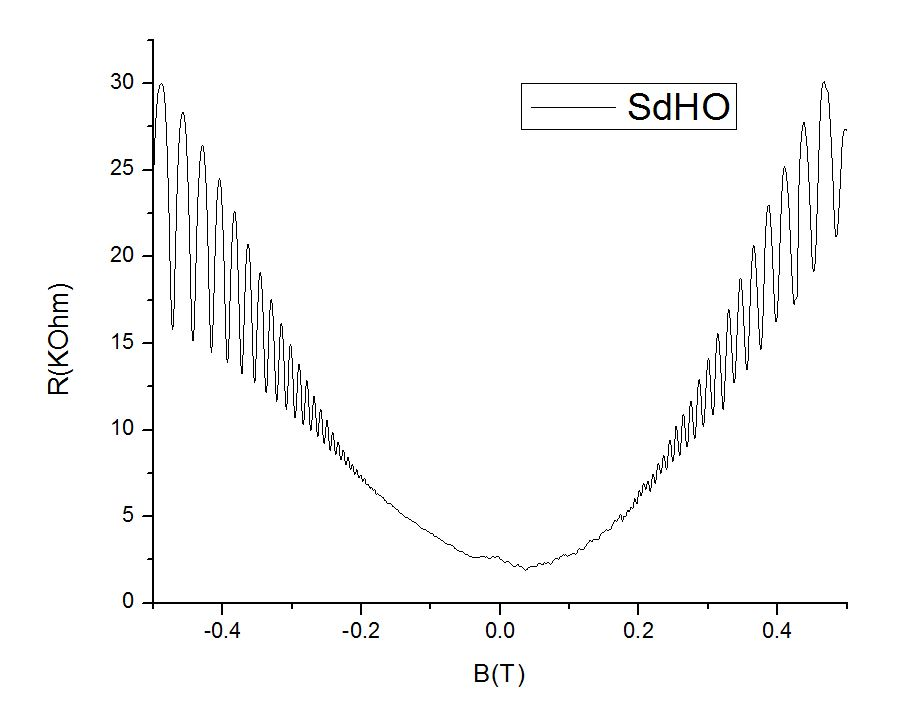
\includegraphics[scale=0.25]{figures/sdho.JPG}
  \caption{Shubnikov de Haas oscillations}
  \label{sdho}
\end{figure}






\section{MIRO and ZRS}\label{MIRO&ZRS}

When microwave is applied, the figure changes quite dramatically.
Additional maximums appear with different intensity at different harmonic peaks which is known as Microwave Induced Resistance Oscillations (MIRO).
MIRO is fascinating nonequilibrium transport phenomenon universal in both n-type and p-type ultrahigh mobility 2D systems. 

\begin{figure}
  \centering
  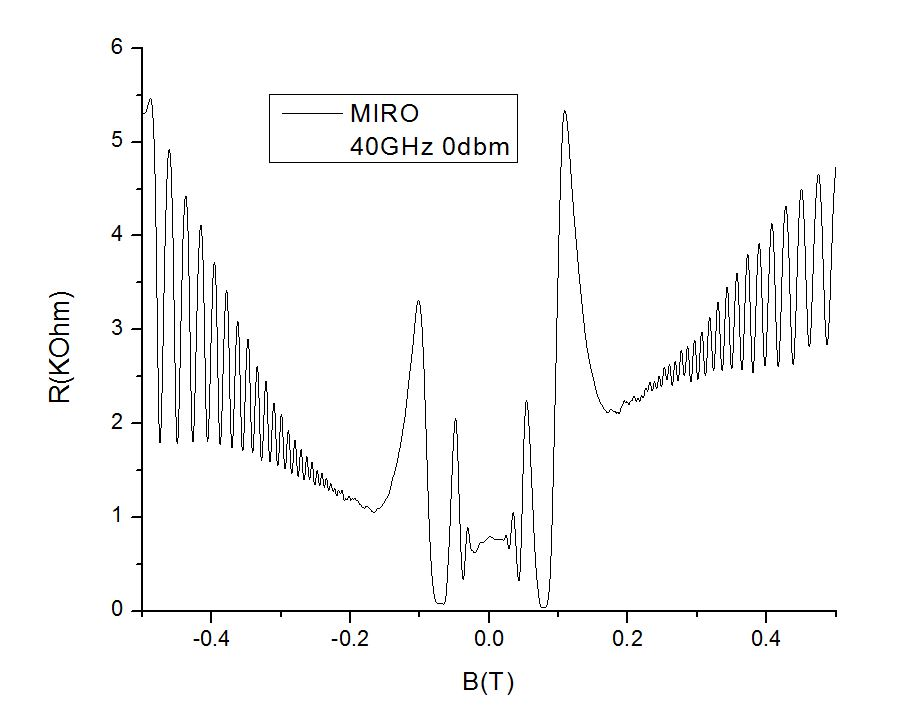
\includegraphics[totalheight=8cm]{figures/miro.JPG}
  \caption{Microwave Induced Resistance Oscillations}
  \label{miro}
\end{figure}
 
Theoretical explanation of MIRO are stated as displacement mechanism and inelastic mechanism [Phys Rev. B 89, 125401 (2014)], both modify the scattering of electrons due to microwave assistance and predict the photoresistance oscillates as 
\begin{align}
\delta R_{\omega}/R_{0} =-2\pi\eta P\lambda^{2}\epsilon \sin(2\pi\epsilon)
\end{align} 
where $\eta$ is the dimensionless scattering rate, $P$ is the dimensionless microwave power, $\lambda$ is the Dingle factor which is related to the quantum lifetime as well as cyclotron frequency and $\epsilon :=\omega/\omega_{c}$. 

Zero resistance state is revealed at the local minimum of MIRO and can be explained as the interaction between microwave and electrons.





\chapter{Thermal detection on behavior of electrons under the illumination of microwave}\label{Thermal}





\section{Theoretical support and preparation in \SI{4}{K}}\label{Theoretical}

As stated in the first chapter, the density of state of 2DEG forms Landau Levels when magnetic field is applied.
Sweeping either microwave frequency or magnetic field will result in the case where energy of the incident photos equal to the energy gap of the Landau Levels, therefore causing resonance phenomenon.
However, in \ce{AlGaAs/GaAs} material, electrons relaxation process can be non-radiative by passing the extra energy to phonons and raising lattice temperature.
This temperature change can be measured by a nano-caloriometer we constructed using special Cernox thermometer which has a huge resistance difference for a tiny temperature change at low temperature.  

\begin{figure}
  \centering
  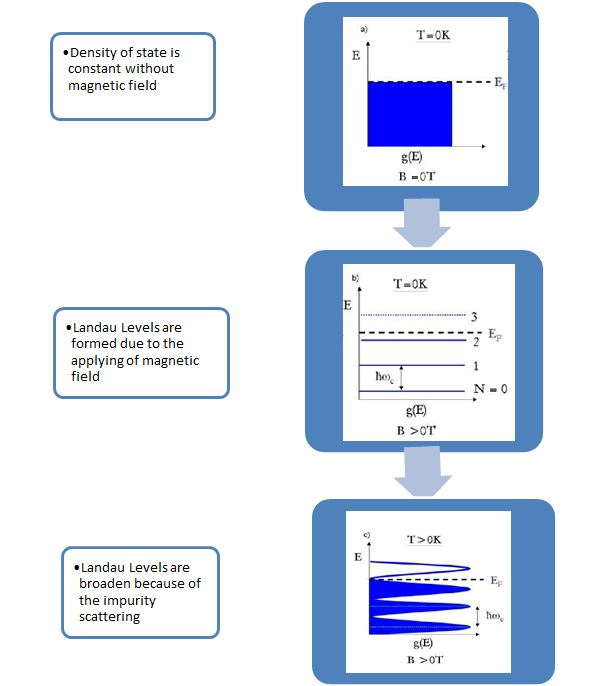
\includegraphics[scale=0.5]{figures/llformation.JPG}
  \caption{Formation of Landau Levels}
  \label{llformation}
\end{figure}
 
\begin{figure}
  \centering
  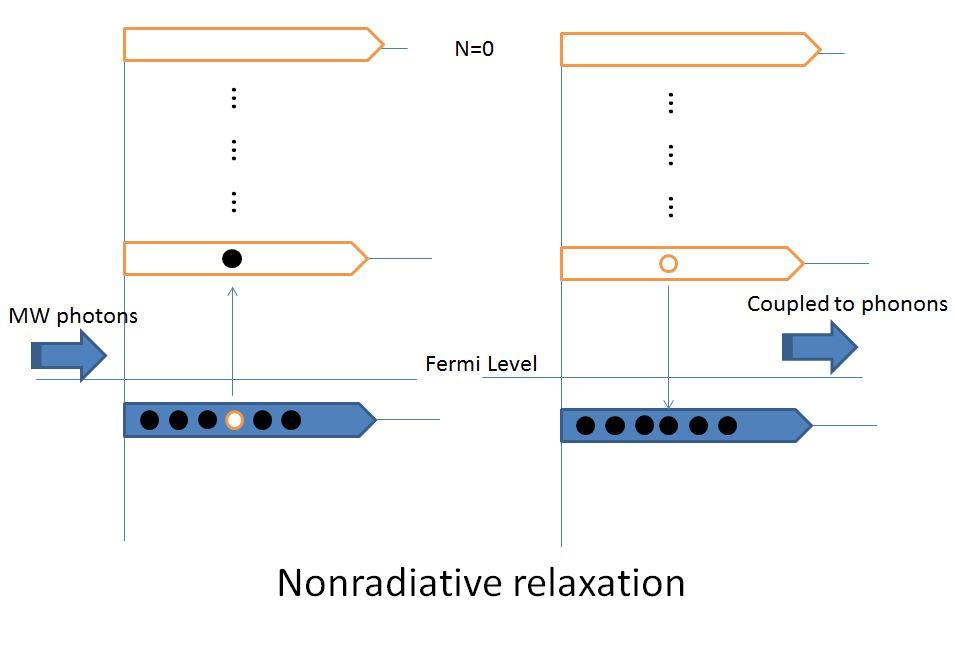
\includegraphics[scale=0.25]{figures/nonradiative.JPG}
  \caption{Non-radiative relaxation}
  \label{nonradiative}
\end{figure}

This resonance measuring method has been tested in our group with liquid helium for detecting geometric resonance which the coupling between cyclotron resonance and plasma resonance. 
On a bare 2DEG chip, cyclotron resonance dips can be resolved clearly.

The coupled frequency can be calculated by the following equation. 

%\begin{figure}
%  \centering
%  \includegraphics[totalheight=8cm]{figures/.JPG}
%  \caption{Non-radiative relaxation}
%  \label{nonradiative}
%\end{figure}

However, on a dot (on the order of \si{\micro\meter}) patterned sample, one can see there are two obvious resonance dips on each side which relate to the plus and minus resonance frequencies shown below.  

%\begin{figure}
%  \centering
%  \includegraphics[totalheight=8cm]{figures/.JPG}
%  \caption{Non-radiative relaxation}
%  \label{nonradiative}
%\end{figure}

\begin{align}
\omega_{\pm}=\frac{\omega_{c}}{2} \pm \sqrt{ \omega_{0}^{2}+ \left(\frac{ \omega_{c} }{2}\right)^{2}}
\end{align}

Here $\displaystyle \omega_{0}^{2}=\frac{N_{s}e^{2}}{2m^{\ast}\epsilon_{\mathrm{eff}}r}$, in our sample, the electron density $N_{s}=2.5\times10^{11}cm^{-2}$, effective mass $m^{*}=0.067m_{e}$, $\epsilon_{\mathrm{eff}}=\frac{1+12}{2}=6.5$ and r is the radius of the dots.

Boundary plasmon has been eliminated by choosing irregularly shaped samples and frequency is limited by the size of our waveguide though it could be extended using frequency multiplier and replacing with coaxial cable. 

 
\section{Setup Construction}\label{Construction}

In order to improve the sensitivity, we constructed another setup which works in \SI{300}{\milli\kelvin} due to the fact that the lower the temperature gets, the shaper resistance line the Cernox thermometer's resistance will act.  

\begin{figure}
  \centering
  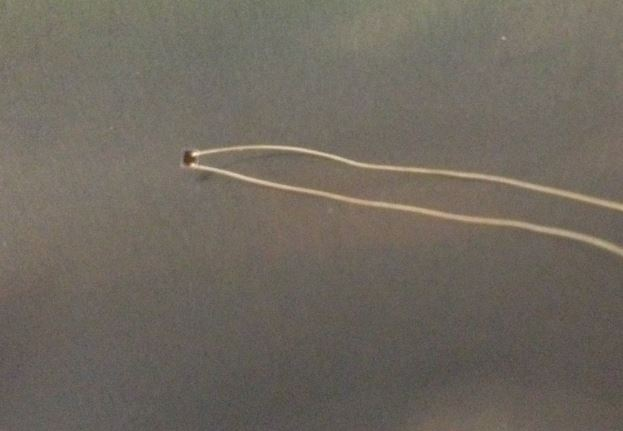
\includegraphics[scale=0.5]{figures/thermometercx.JPG}
  \caption{Cernox thermometer}
  \label{thermometer}
\end{figure}
 
 
However, going from \SI{4}{\kelvin} to \SI{300}{\milli\kelvin} is a big leap and there are problems that we have to overcome.
The most significant one is sealing in \ce{^{3}He} liquid environment.
Since the heat generated by the non-radiative relaxation is very small, the sample need to be in vacuum to avoid being carried away by massive \ce{^{3}He} liquid and a high heat conductive media to pass the temperature change to the thermometer.
Meanwhile, to keep the temperature around \SI{300}{\milli\kelvin}, we need something with low heat conductivity to connect the inside setup to outside.
In this case, we use thin sapphire crystal as the bridge between sample and thermometer, thin magnin wire for keeping vacuum temperature low. 
 

\begin{figure}
  \centering
  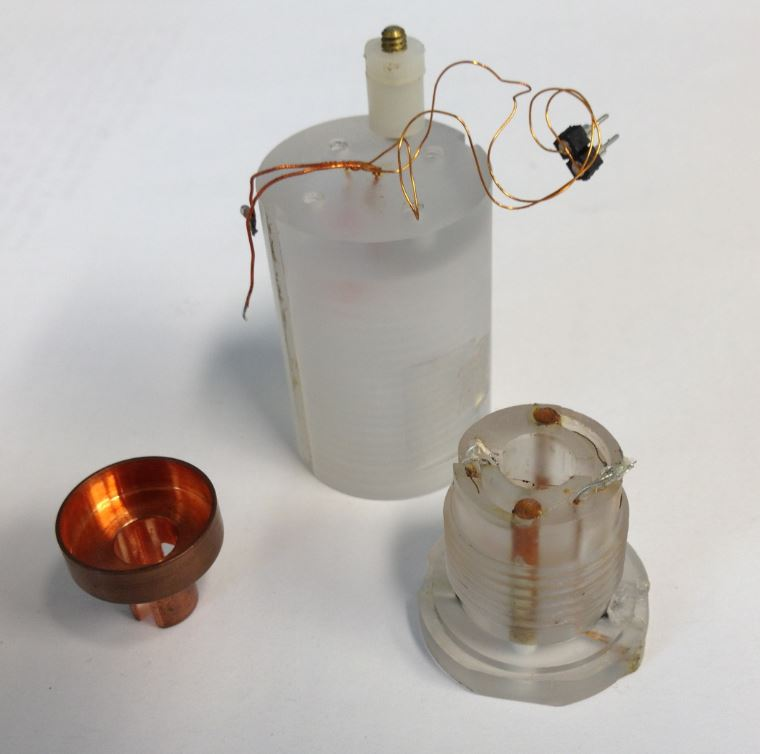
\includegraphics[scale=0.5]{figures/vacuumcan.JPG}
  \caption{1266 Epoxy vacuum can}
  \label{vacuum-can}
\end{figure}
 
 

\begin{figure}
  \centering
  \includegraphics[scale=0.5]{figures/SCHEMA.JPG}
  \caption{Thermal detection setup schema}
  \label{thermal-schema}
\end{figure}
 
 
\begin{figure}
  \centering
  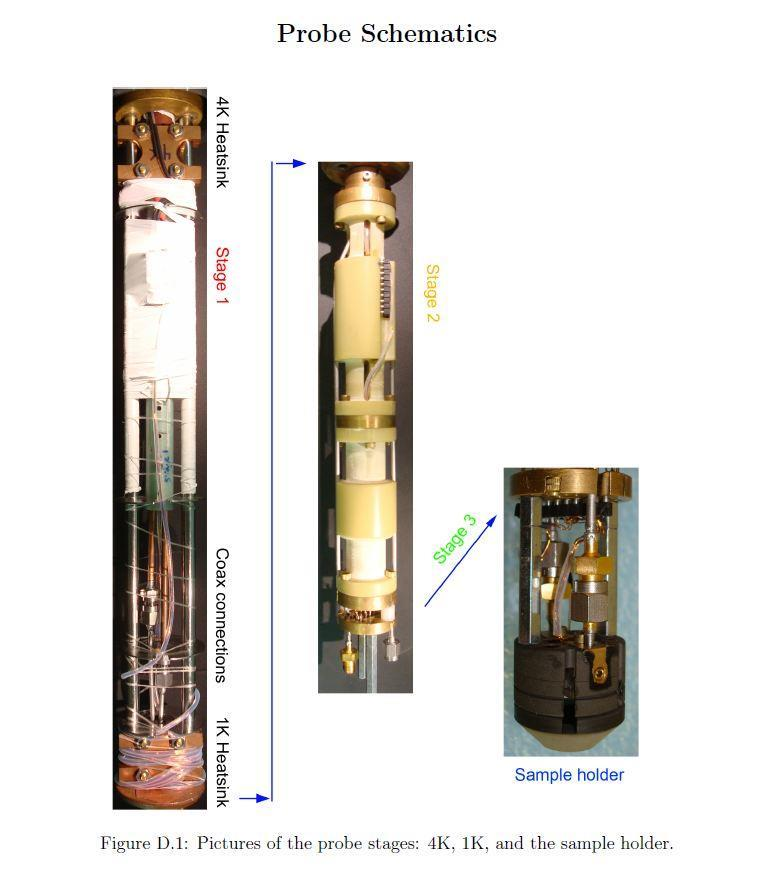
\includegraphics[scale=0.5]{figures/probe.JPG}
  \caption{\ce{^{3}He} top loaded Refrigerator coaxial probe}
  \label{probe}
\end{figure}

\section{Cyclotron Resonance Pretest}\label{Cyclotron}

\begin{figure}
  \centering
  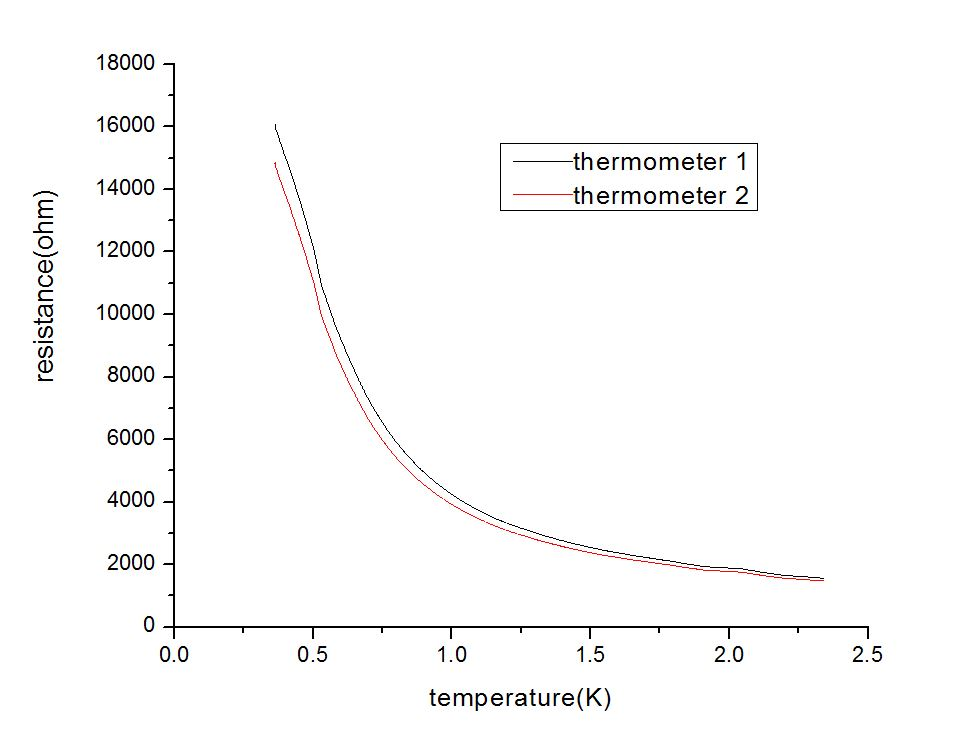
\includegraphics[scale=0.5]{figures/R(T).JPG}
  \caption{Temperature dependence of the thermometers}
  \label{r(t)}
\end{figure}
 
 
\begin{figure}
  \centering
  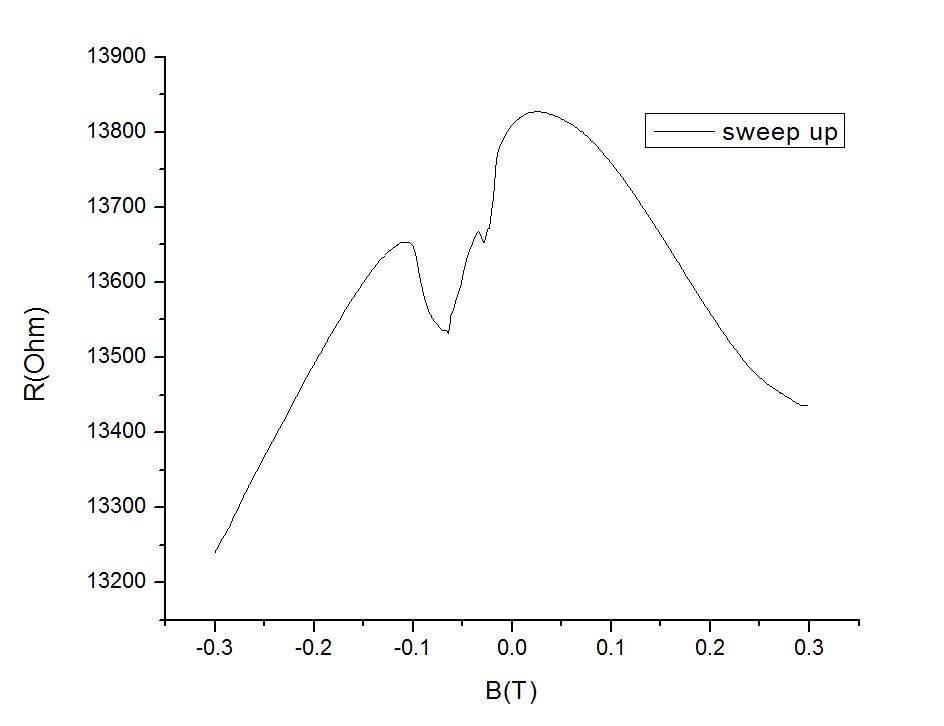
\includegraphics[scale=0.5]{figures/R(B)UP.JPG}
  \caption{Background sweeping}
  \label{r(b)}
\end{figure}

\begin{figure}
  \centering
  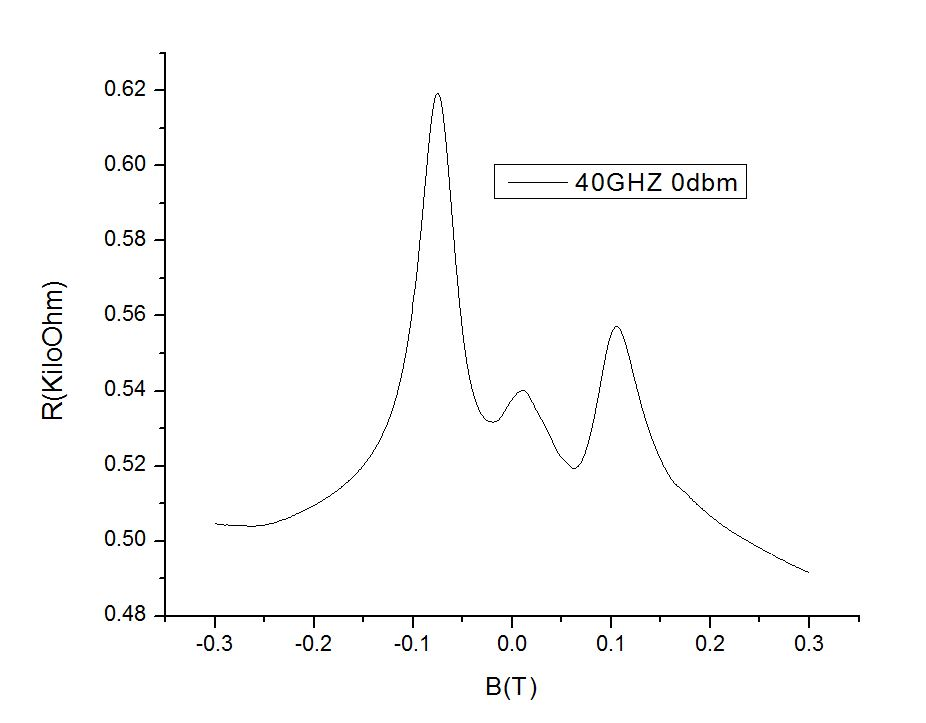
\includegraphics[scale=0.5]{figures/0dbm.JPG}
  \caption{CR at 0dbm 40GHz}
  \label{0dbm_40ghz}
\end{figure}
 
 
\begin{figure}
  \centering
  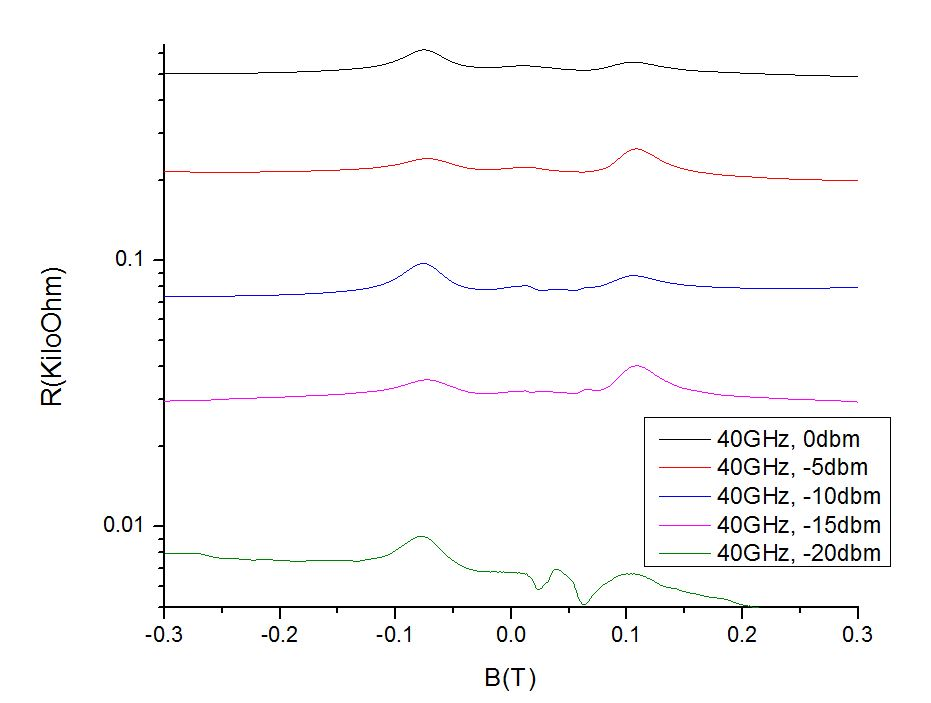
\includegraphics[scale=0.5]{figures/thermopowerdep.JPG}
  \caption{Power dependence}
  \label{thermopowerdep}
\end{figure}
 






\section{Spin Resonance on DPPH}\label{DPPH}


\begin{figure}
  \centering
  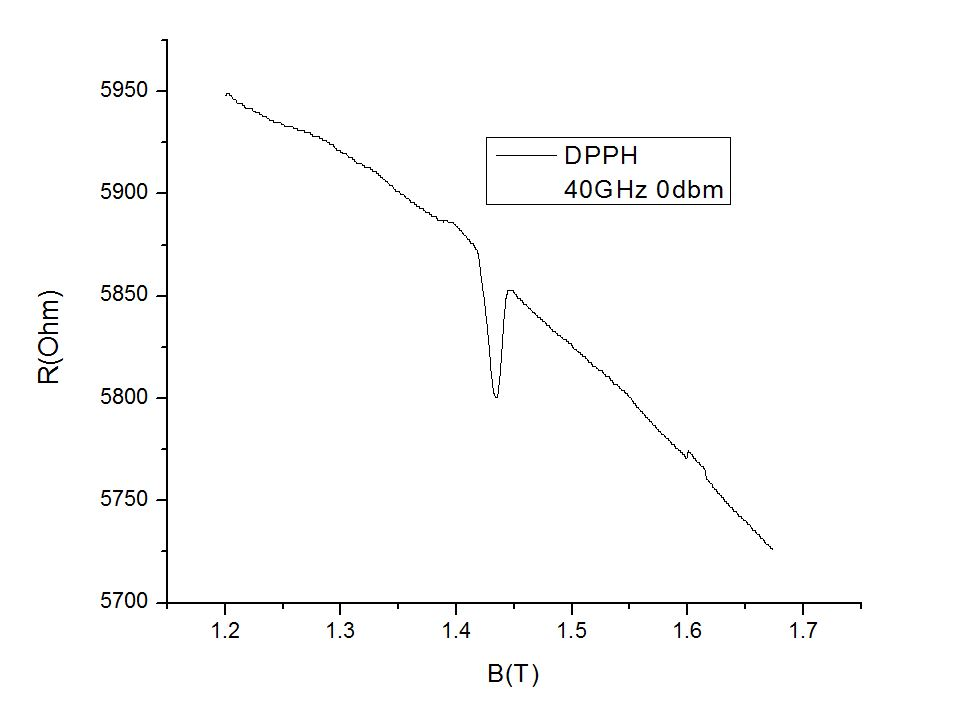
\includegraphics[scale=0.5]{figures/dpph_esr.JPG}
  \caption{ESR of DPPH}
  \label{dpph_esr}
\end{figure}
 
 
\begin{figure}
  \centering
  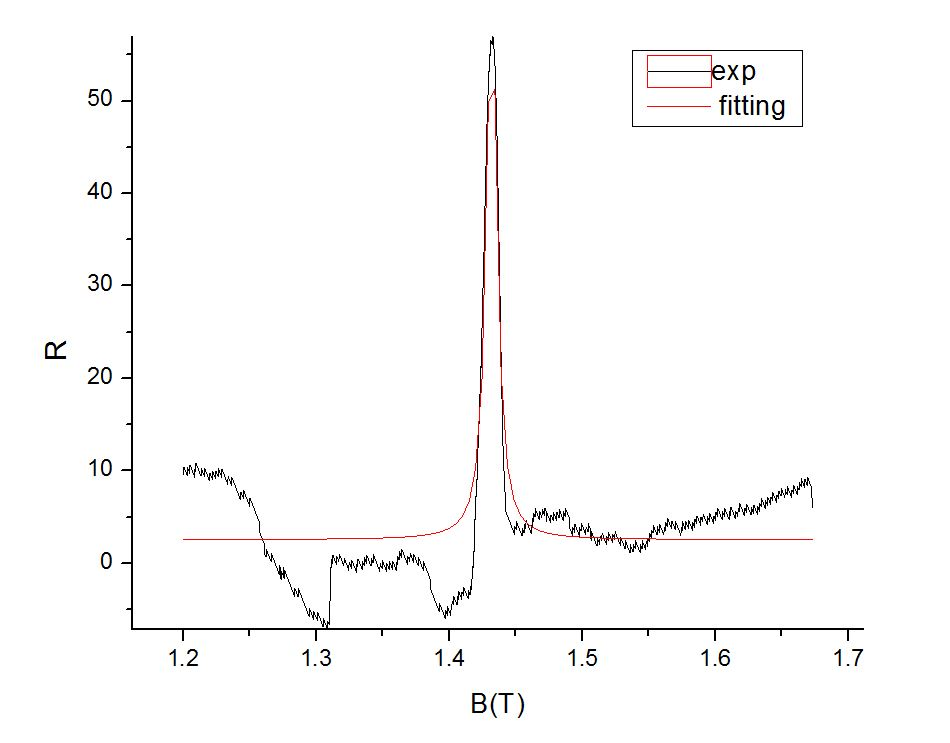
\includegraphics[scale=0.5]{figures/dpph_fitting.JPG}
  \caption{ESR Fitting of DPPH}
  \label{dpph_fitting}
\end{figure}
 









\chapter{Microwave absorption spectroscopy of electrons in 2DEG}\label{Absorption}




\section{Setup Construction}\label{Construction}

\begin{figure}
  \centering
  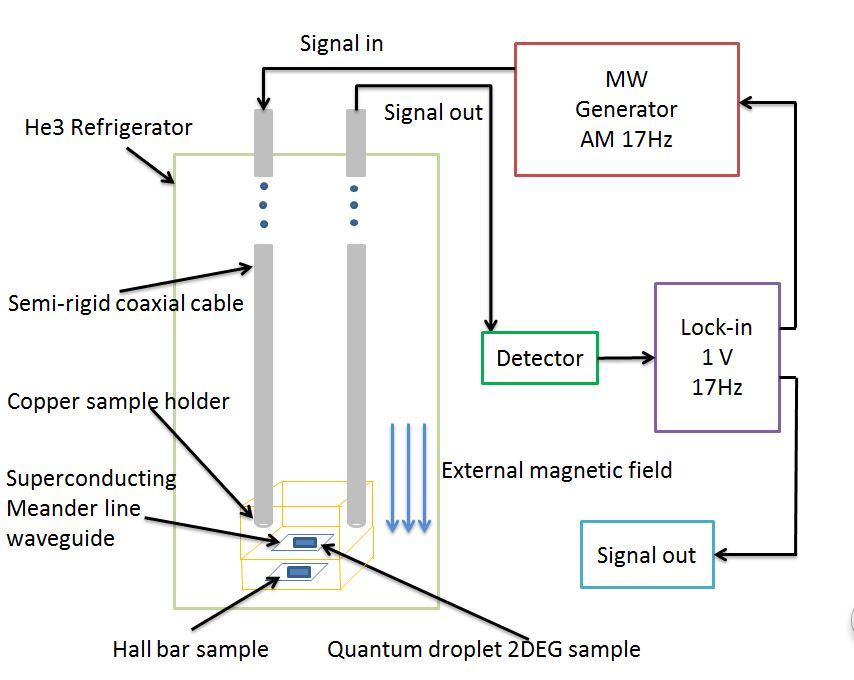
\includegraphics[scale=0.5]{figures/configuration.JPG}
  \caption{Microwave absorption spectroscopy construction}
  \label{configuration}
\end{figure}
 
 
 
 
 
 
 

\section{Cyclotron Resonance Pretest}\label{Cyclotron}

\begin{figure}
  \centering
  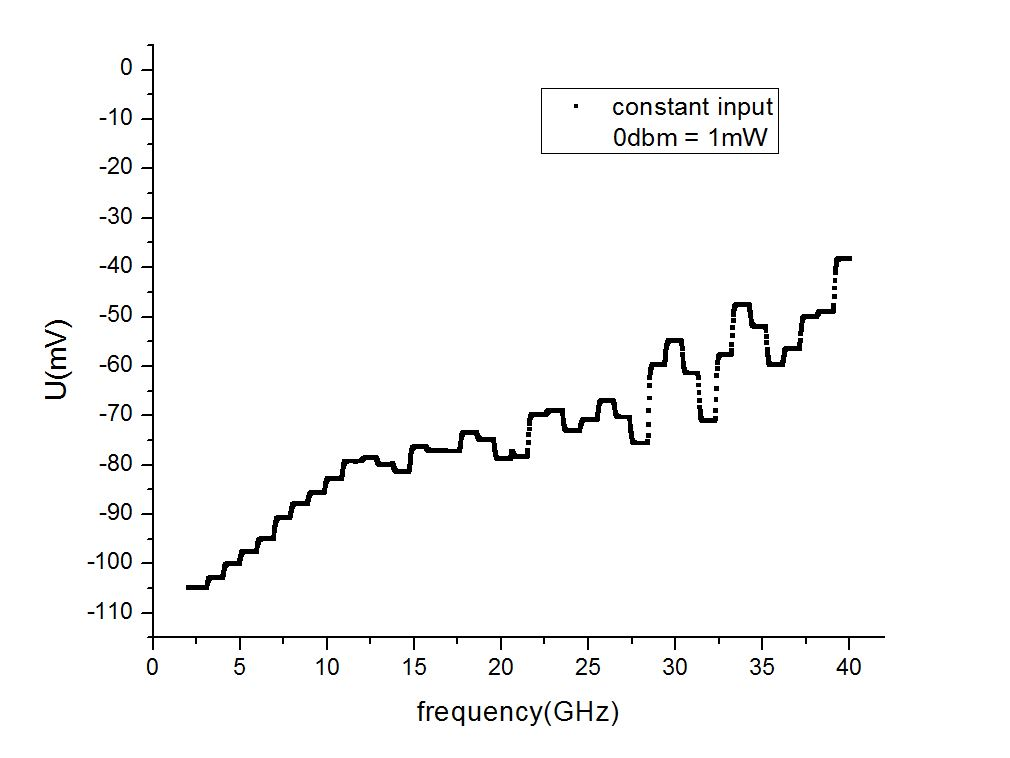
\includegraphics[totalheight=8cm]{figures/spec.JPG}
  \caption{setup calibration 1}
  \label{spec}
\end{figure}
 

\begin{figure}
  \centering
  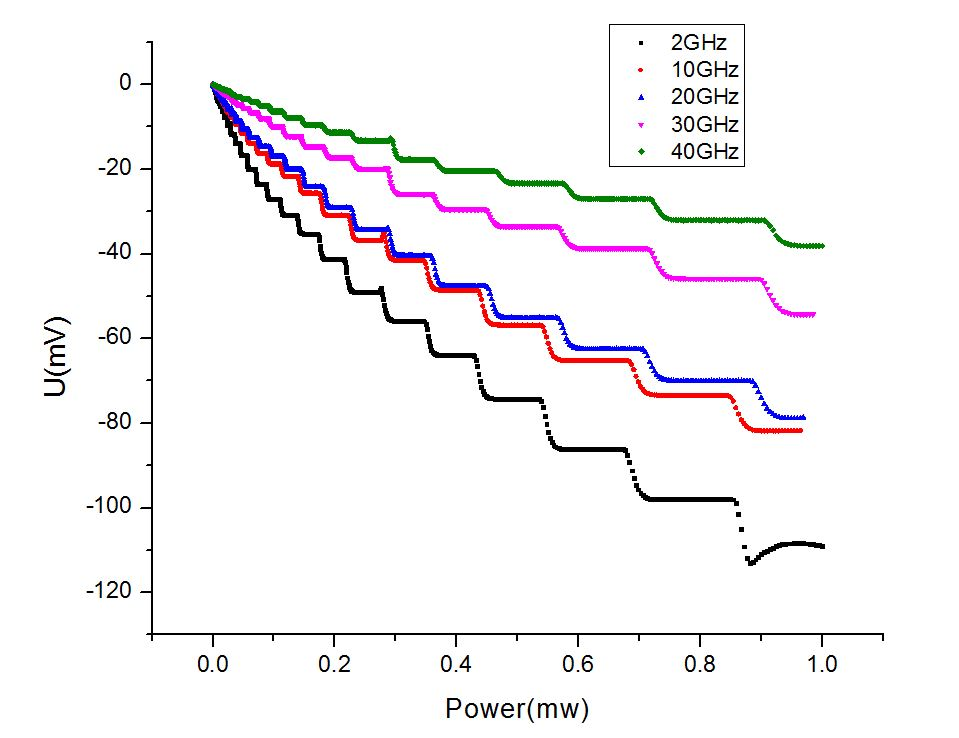
\includegraphics[totalheight=8cm]{figures/multifre.JPG}
  \caption{setup calibration 2}
  \label{multifre}
\end{figure}
 

\begin{figure}
  \centering
  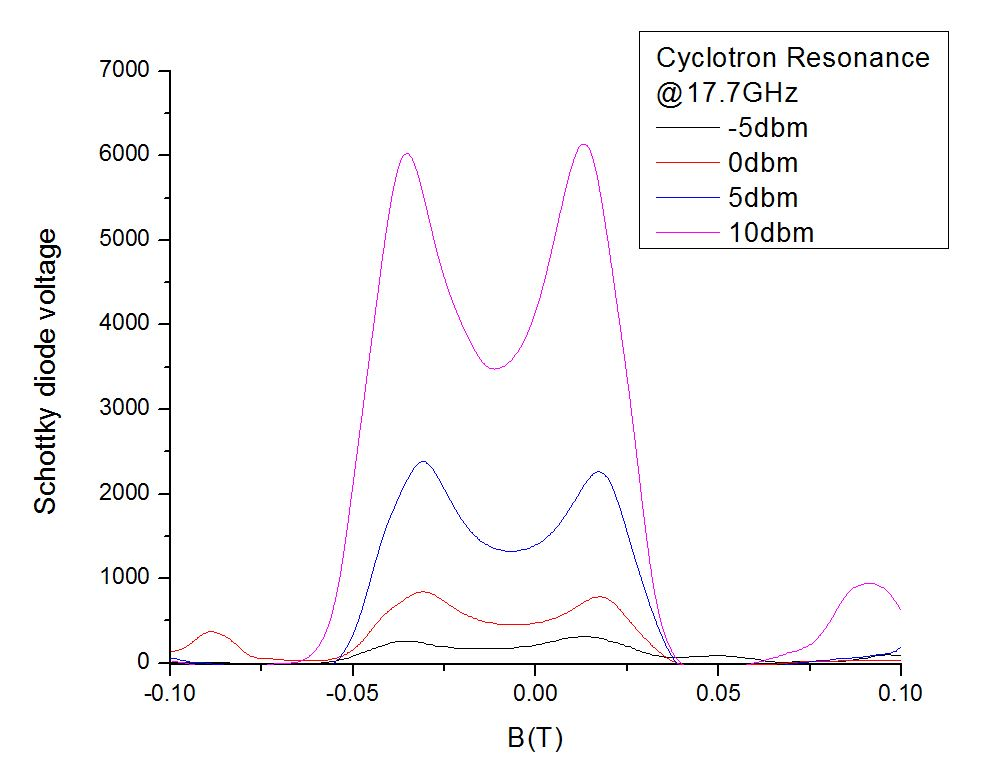
\includegraphics[totalheight=8cm]{figures/CRpowerdep.JPG}
  \caption{cyclotron pretest}
  \label{crpowerdep}
\end{figure}
 







\section{Improvement underway}\label{Improvement}






\chapter{Summary}\label{summary}





\appendix

%\include{append-a}
%\appendix
%\addcontentsline{toc} {chapter}{\numberline {}Appendix A}
%\include{append-a}
%\include{append-b}
%\addcontentsline{toc} {chapter}{\numberline {}Bibliography}{}
%\include{biblio}

\bibliographystyle{ieeetr}
\bibliography{Jie Zhang}
\end{document}
